\documentclass[11pt,letterpaper]{article}
\usepackage[utf8]{inputenc}
\usepackage{amsmath,amssymb,fullpage,graphicx}
\usepackage{afterpage}

\begin{document}
\subsection*{Lect 15-4}
\subsection*{a}
\begin{verbatim}
library(AlgDesign)
rm(list=ls(all=TRUE))
design <- gen.factorial(c(2,2,4), varNames = c('A', 'B', 'Replication'), factors = 'all')
attach(design)
y <- c(18.2,27.2,15.9,41,18.9,24,14.5,43.9,12.9,22.4,15.1,36.3,14.4,22.5,14.2,39.9)

lm1 <- lm(y~A + B + A:B)
summary.aov(lm1)

            Df Sum Sq Mean Sq F value   Pr(>F)    
A            1 1107.2  1107.2  185.25 1.17e-08 ***
B            1  227.3   227.3   38.02 4.83e-05 ***
A:B          1  303.6   303.6   50.80 1.20e-05 ***
Residuals   12   71.7     6.0                     
---
\end{verbatim}

\subsection*{b}
\begin{verbatim}
n <- 4
data1 <- data.frame(cbind(y, A, B, Replication))
yate_1 <- sum(data1[A==1 & B==1,1])
yate_a <- sum(data1[A==2 & B==1,1])
yate_b <- sum(data1[A==1 & B==2,1])
yate_ab <- sum(data1[A==2 & B==2,1])

SSA <- (-yate_1 + yate_a - yate_b + yate_ab)^2 / (4 * n)
SSB <- (-yate_1 - yate_a + yate_b + yate_ab)^2 / (4 * n)
SSAB <- (yate_1 - yate_a - yate_b + yate_ab)^2 / (4 * n)
SST <- sum((y - mean(y))^2)
SSE <- SST - SSA - SSB - SSAB

c(SSA, SSB, SSAB, SSE)
[1] 1107.2256  227.2556  303.6306   71.7225
\end{verbatim}

\subsection*{c}
\begin{verbatim}
par(mfrow=c(1,2))
ylimit <- c(min(y), max(y))

par(mfrow=c(1,1))
boxplot(data1[A==1 & B==1,1],data1[A==2 & B==1,1], ylim=ylimit, 
        xlab='A-/A+, left/right', main='B-/B+, white/red')
boxplot(data1[A==1 & B==2,1],data1[A==2 & B==2,1],add=T,col='red',boxwex=0.5)
\end{verbatim}

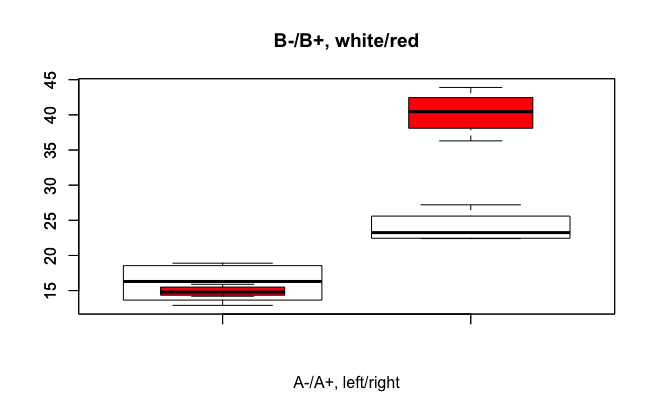
\includegraphics[scale=0.55]{lect-15-4-c-2.png}

\noindent Base on the boxplot of combination of A B levels, we can see the combination of A=- and B=+ has the smallest median and narrowest range. A=- denotes 1/16 bit size, B=+ denotes 90 rpm, and Y value denotes vibration. Since we want less vibration, I will operate under 1/16 bit size and 90 rpm. \\

\subsection*{d}
\noindent Drawing two lines to connect median value of two red boxes and connect median value of two white boxes, we can see the slopes of two connecting line is different. This implies the interaction between A and B exists. 
\newpage
\subsection*{Lect 16-4}
\subsection*{a}
\begin{verbatim}
rm(list=ls(all=TRUE))
design2 <- gen.factorial(c(2,2,2,2,2), varNames = c('A','B', 'C', 'D','Rep'))
attach(design2)
y2 <- c(7.037, 14.707, 11.635, 17.273, 10.403, 4.368, 9.360, 13.440, 8.561, 16.867, 13.876, 
        19.824, 11.846, 6.125, 11.190, 15.653, 6.376, 15.219, 12.089, 17.815, 10.151, 4.098, 
        9.253, 12.923, 8.951, 17.052, 13.658, 19.639, 12.337, 5.904, 10.935, 15.053)
data2 <- data.frame(y2,A,B,C,D)
lm2 = lm(y2~A*B*C*D)
anovatable <- summary.aov(lm2)[[1]]
MSE <- anovatable$`Mean Sq`[16]
summary.aov(lm2)

            Df Sum Sq Mean Sq  F value   Pr(>F)    
A            1  72.91   72.91  898.339 1.74e-15 ***
B            1 126.46  126.46 1558.172  < 2e-16 ***
C            1 103.46  103.46 1274.822  < 2e-16 ***
D            1  30.66   30.66  377.802 1.49e-12 ***
A:B          1  29.93   29.93  368.739 1.79e-12 ***
A:C          1 128.50  128.50 1583.256  < 2e-16 ***
B:C          1   0.07    0.07    0.908    0.355    
A:D          1   0.05    0.05    0.577    0.459    
B:D          1   0.02    0.02    0.220    0.645    
C:D          1   0.05    0.05    0.583    0.456    
A:B:C        1  78.75   78.75  970.325 9.49e-16 ***
A:B:D        1   0.08    0.08    0.947    0.345    
A:C:D        1   0.00    0.00    0.036    0.852    
B:C:D        1   0.01    0.01    0.125    0.728    
A:B:C:D      1   0.00    0.00    0.020    0.890    
Residuals   16   1.30    0.08                      
---
\end{verbatim}

\noindent From the ANOVA table, we may perceive that factors $A, B, C, D$ and interactions $AB, AC, ABC$ have significant effects, because their F-test p-values are extremely small. Among these significant factors, $B, C, AC$ are most significant for their SS's are relatively larger than other SS's.

\subsection*{b}
\begin{verbatim}
contr <- as.character("contr.helmert")
lm3 <- lm(y2~A*B*C*D, contrasts = list(A1=contr,B1=contr,C1=contr,D1=contr))
summary.lm(lm3) 
             Estimate Std. Error t value Pr(>|t|)    
(Intercept) 11.988062   0.050361 238.042  < 2e-16 ***
A            1.509438   0.050361  29.972 1.74e-15 ***
B            1.987938   0.050361  39.474  < 2e-16 ***
C           -1.798125   0.050361 -35.705  < 2e-16 ***
D            0.978875   0.050361  19.437 1.49e-12 ***
A:B          0.967062   0.050361  19.203 1.79e-12 ***
A:C         -2.003875   0.050361 -39.790  < 2e-16 ***
B:C          0.048000   0.050361   0.953    0.355    
A:D          0.038250   0.050361   0.760    0.459    
B:D          0.023625   0.050361   0.469    0.645    
C:D         -0.038438   0.050361  -0.763    0.456    
A:B:C        1.568750   0.050361  31.150 9.49e-16 ***
A:B:D        0.049000   0.050361   0.973    0.345    
A:C:D        0.009563   0.050361   0.190    0.852    
B:C:D        0.017813   0.050361   0.354    0.728    
A:B:C:D      0.007062   0.050361   0.140    0.890  

all_effects <- 2 * (lm3$coefficients)[-1]

> all_effects
        A         B         C         D       A:B       A:C       B:C       A:D 
 3.018875  3.975875 -3.596250  1.957750  1.934125 -4.007750  0.096000  0.076500 
      B:D       C:D     A:B:C     A:B:D     A:C:D     B:C:D   A:B:C:D 
 0.047250 -0.076875  3.137500  0.098000  0.019125  0.035625  0.014125 
 
\end{verbatim}

\subsection*{c}
\noindent Note that $Contrast(A) = Y_{2....} - Y_{1....}$, $Contrast(AB) = Y_{22...} - Y_{11...}$ and etc. Also, the +/- of each term in $Contrast(AB)$ is determined by multiplying +/- of terms in $Contrast(A)$ and $Constrast(B)$.

\begin{verbatim}
contrasts_15 <- apply(y2*cbind(A, B, C, D, A*B, A*C, A*D,
                            B*C,B*D, C*D, A*B*C, A*B*D, A*C*D, B*C*D, A*B*C*D), 2, sum)

> contrasts_15
      A       B       C       D                                                 
 48.302  63.614 -57.540  31.324  30.946 -64.124   1.224   1.536   0.756  -1.230 
                                        
 50.200   1.568   0.306   0.570   0.226 
\end{verbatim}

\subsection*{d}
\begin{verbatim}
k <- 4
n <- 2
p <- 15 + 1
effects_15 <- 1/(2^(k-1)*n)*contrasts_15
t_obs_15 <- effects_15 / sqrt(MSE/(2^(k-2)*n))
p_values_15 <- 2*pt(abs(t_obs_15), df=2^k*n - p, lower.tail = F)
t_tests_byhand <- cbind(effects_15, t_obs_15, p_values_15)
colnames(t_tests_byhand) <- c('effects', 't-stats', 'p-values')
rownames(t_tests_byhand) <- c('A','B','C','D','AB','AC','AD','BC','
                              BD','CD','ABC','ABD','ACD','BCD','ABCD')
                              
t_tests_byhand
     effects_15    t_obs_15  p_values_15
A      3.018875  29.9723026 1.740225e-15
B      3.975875  39.4736876 2.247046e-17
C     -3.596250 -35.7046559 1.100354e-16
D      1.957750  19.4371332 1.485334e-12
AB     1.934125  19.2025770 1.790240e-12
AC    -4.007750 -39.7901522 1.979949e-17
AD     0.076500   0.7595151 4.585895e-01
BC     0.096000   0.9531170 3.547091e-01
BD     0.047250   0.4691123 6.453180e-01
CD    -0.076875  -0.7632382 4.564284e-01
ABC    3.137500  31.1500474 9.485296e-16
ABD    0.098000   0.9729736 3.450474e-01
ACD    0.019125   0.1898788 8.517922e-01
BCD    0.035625   0.3536958 7.281845e-01
ABCD   0.014125   0.1402373 8.902228e-01
\end{verbatim}

\noindent The result of effect t-test that is calculated by hand is similar to result from $lm()$ function. By t-test, p-value shows significant evidence to reject the null hypothesis that A or B or C or D or AB or AC or ABC has no effects. 

\subsection*{e}
\begin{verbatim}
contr <- as.character("contr.helmert")
lm3 <- lm(y2~A*B*C*D, contrasts = list(A=contr,B=contr,C=contr,D=contr))
summary.lm(lm3) 
effs <- 2 * (lm3$coefficients)[-1]
as.matrix(effs,col=1)
             [,1]
A        3.018875
B        3.975875
C       -3.596250
D        1.957750
A:B      1.934125
A:C     -4.007750
B:C      0.096000
A:D      0.076500
B:D      0.047250
C:D     -0.076875
A:B:C    3.137500
A:B:D    0.098000
A:C:D    0.019125
B:C:D    0.035625
A:B:C:D  0.014125
\end{verbatim}

\noindent From the table of effects, we can perceive A,B,D,AB,ABC have the highest 5 effects, while C,AC have smallest effects (negative effects). 

\begin{verbatim}
qqnorm(effs)
abline(median(effs), MSE, lty=2, col=2)
\end{verbatim}
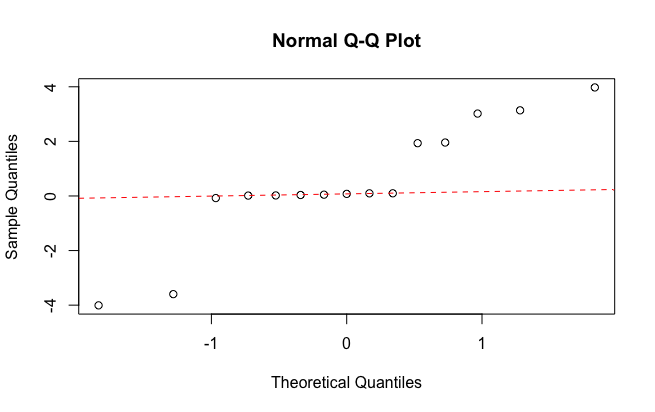
\includegraphics[scale=0.55]{lect-16-4-e.png}

\noindent  We can see 5 effects at highest quantile and 2 effects at lowest quantile are excluded from linear pattern, implying they are significant to have effects. Match the effect table to normal qqplot of effects, we can see the significant effects are A,B,C,D,AB,AC,ABC factors. The result is same as above. 

\newpage
\subsection*{Lect 17-2}
\subsection*{a}
\begin{verbatim}
rm(list=ls(all=T))
design4 <- gen.factorial(c(2,2,3), varNames = c('A','B','RR'))
attach(design4)
rep1 <- c(28,36,18,31)
rep2 <- c(25,32,19,30)
rep3 <- c(27,32,23,29)
y4 <- c(rep1,rep2,rep3)
contr <- as.character("contr.helmert")
A <- as.factor(A)
B <- as.factor(B)
lm4 <- lm(y4~A*B, contrasts = list(A=contr, B=contr))

> summary.aov(lm4)
            Df Sum Sq Mean Sq F value   Pr(>F)    
A            1 208.33  208.33  53.191 8.44e-05 ***
B            1  75.00   75.00  19.149  0.00236 ** 
A:B          1   8.33    8.33   2.128  0.18278    
Residuals    8  31.33    3.92                     
---

effects4 <- 2 * lm4$coefficients[-1]
> effects4
        A         B       A:B 
 8.333333 -5.000000  1.666667 
\end{verbatim}

\subsection*{b}
\begin{verbatim}
RR <- RR + 2
BL <- as.factor(RR)
lm5 <- lm(y4~A + B + A*B + BL, contrasts = list(A=contr,B=contr, BL=contr))

> summary.aov(lm5)
            Df Sum Sq Mean Sq F value   Pr(>F)    
A            1 208.33  208.33  50.336 0.000394 ***
B            1  75.00   75.00  18.121 0.005340 ** 
BL           2   6.50    3.25   0.785 0.497835    
A:B          1   8.33    8.33   2.013 0.205710    
Residuals    6  24.83    4.14                 
---

effects5 <- 2 * lm5$coefficients[-1]
> effects5
       A1        B1       BL1       BL2     A1:B1 
 8.333333 -5.000000 -1.750000  0.250000  1.666667 
\end{verbatim}

\subsection*{c}
\noindent Compare to the CRD ANOVA table, the SSE on RCBD ANOVA table is smaller, because SSE in CRD equals sum of SSE and SSBL in RCBD. However, the p-value in CRD is smaller than RCBD, since the degree of freedom of residuals in RCBD (6) is smaller than CRD (8). 

\subsection*{d}
\begin{verbatim}
sse_obs <- summary.aov(lm5)[[1]][5,2]
y.m <- matrix(c(rep1,rep2,rep3), ncol=3, byrow=F)
ntrials <- 5000
set.seed(123)
sse_sample <- numeric(ntrials)
for (i in 1:ntrials) {
  new_y.m <- t(apply(t(y.m),2,sample))
  lm_temp <- lm(as.vector(new_y.m)~A+B+A*B+BL)
  sse_temp <- summary.aov(lm_temp)[[1]][5,2]
  sse_sample[i] <- sse_temp
}
hist(sse_sample, main='Empirical Distribution of SSE under H0', 
     xlab='Sample SSE', probability = T)
\end{verbatim}
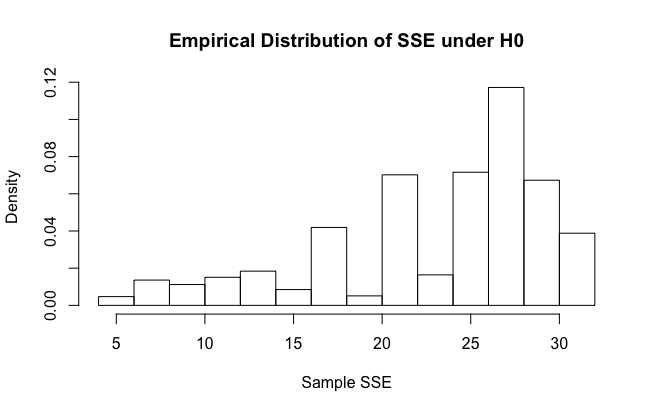
\includegraphics[scale=0.55]{lect-17-2-d.png}

\subsection*{e}
\begin{verbatim}
sse_p_value <- length(sse_sample[sse_sample <= sse_obs]) / ntrials

> sse_p_value
[1] 0.464
\end{verbatim}

\noindent P-value is the probability of getting extreme value under the null hypothesis. The null hypothesis states block has no effect, i.e. SSE in RCBD should be equal to SSE in CRD. To find evidence against the null, we need evidence that SSB greater than zero, i.e. SSE in RCBD should be less than SSE in CRD. Therefore, it is a one-sided test on lower tail. \\

\noindent In the empirical distribution, there are $46.4 \%$ sample data less than observed SSE. The p-value of observed SSE under the null is 0.464.

\subsection*{f}
\begin{verbatim}
rm(list=ls(all=TRUE))
rep1 <- c(28,36,18,31)
rep2 <- c(25,32,19,30)
y6 <- c(rep1, rep2)
design6 <- gen.factorial(c(2,2,2), varNames = c('A','B','RR'))
attach(design6)
A <- as.factor(A)
B <- as.factor(B)
lm6 <- lm(y6~A*B)

> summary.aov(lm6)
            Df Sum Sq Mean Sq F value  Pr(>F)   
A            1 190.13  190.13   56.33 0.00169 **
B            1  66.12   66.12   19.59 0.01145 * 
A:B          1  10.12   10.12    3.00 0.15830   
Residuals    4  13.50    3.37                   
---
\end{verbatim}

\subsection*{g}
\begin{verbatim}
BL <- numeric(length(y6))
BL[B==-1] <- 1
BL[B==1] <- 2
BL <- as.factor(BL)
lm7 <- lm(y6~A+B+A*B + BL)

> summary.aov(lm7)
            Df Sum Sq Mean Sq F value  Pr(>F)   
A            1 190.13  190.13   56.33 0.00169 **
B            1  66.12   66.12   19.59 0.01145 * 
A:B          1  10.12   10.12    3.00 0.15830   
Residuals    4  13.50    3.37                   
---
\end{verbatim}

\subsection*{h}
\noindent The ANOVA table in part g and part f are exactly same, because effect of B is confounded with block effect. 


\end{document}